\documentclass{article}
\usepackage[margin=2.5cm, top=4cm, headheight=25pt]{geometry}
\usepackage{amsmath, amssymb, enumitem, fancyhdr, graphicx}
\usepackage[indent=20pt]{parskip}
\usepackage[hidelinks]{hyperref}
\usepackage{xcolor}
\usepackage{listings}
\usepackage{subcaption}
\usepackage{url}
\usepackage[most]{tcolorbox}
\usepackage{lastpage}

\tcbuselibrary{listingsutf8} % Support for lstlistings within tcolorbox

\newtcolorbox[auto counter, number within=section]{question}[1][]{%
    colframe=gray!80,                      % Dark gray frame
    colback=gray!5,                       % Light gray background
    coltitle=black,                        % Black title
    title=\textbf{Question~\thetcbcounter}, % Bold title
    fonttitle=\bfseries\large,             % Subtle title font size
    rounded corners,                   % Slightly more rounded corners
    boxrule=0.25mm,                         % Thinner border for a sleek look
    enhanced,                              % Enhanced box features
    attach boxed title to top left={xshift=2mm, yshift=-2mm},
    boxed title style={colframe=gray!80, colback=gray!5, boxrule=0.25mm},
    % Title styling
    #1
}

\bibliographystyle{IEEEtran}
\graphicspath{{./images/}}

% -- Custom Variables --
\def\me{Rajdeep Gill 7934493}
\def\course{ECE 3700}
\def\labsection{B01}
\def\labno{1}
\def\title{Wireshark Lab}

% -- Styling for code snippets --
\lstset{
    basicstyle=\ttfamily\small,           % Basic font style
    keywordstyle=\color{blue},            % Keywords color
    commentstyle=\color{gray},            % Comments color
    stringstyle=\color{teal},             % Strings color
    numbers=left,                         % Line numbers on the left
    numberstyle=\tiny\color{gray},        % Line number style
    stepnumber=1,                         % Line number step
    numbersep=10pt,                       % Space between line numbers and code
    backgroundcolor=\color{lightgray!10}, % Background color
    frame=single,                         % Adds a frame around the code
    breaklines=true,                      % Line breaking for long lines
    captionpos=b,                         % Caption position
    showspaces=false,                     % Don't show spaces
    showstringspaces=false                % Don't show spaces in strings
}
\renewcommand{\lstlistingname}{Code Snippet}

\renewcommand{\arraystretch}{1.2} % For less-ugly tables
\setlength\parindent{0pt}

%----- Samples 
% Questions:
%   \begin{question}[title=Custom Question Title]
%       Question details
%   \end{question}

% Tables:
%   \begin{table}[htbp]
%       \centering
%       \caption{Table Caption}
%       \begin{tabular}{ll}
%           \toprule
%           \textbf{Column 1} & \textbf{Column 2} \\
%           \midrule
%           Row 1 & Row 2 \\
%           Row 3 & Row 4 \\
%           \bottomrule
%       \end{tabular}
%   \end{table} 

% Figures:
%   Single figure:
%       \begin{figure}[htbp]
%           \centering
%           \includegraphics[width=0.5\textwidth]{example-image}
%           \caption{Figure Caption}
%       \end{figure}
%   Multiple figures:
%       \begin{figure}[htbp]
%           \centering
%           \begin{subfigure}[b]{0.5\textwidth}
%               \includegraphics[width=\textwidth]{example-image-a}
%               \caption{First subfigure}
%           \end{subfigure}
%           \begin{subfigure}[b]{0.5\textwidth}
%               \includegraphics[width=\textwidth]{example-image-b}
%               \caption{Second subfigure}
%           \end{subfigure}
%           \caption{Main figure}
%       \end{figure}

\begin{document}

% --------------------------------------------------------------------------------
% TITLE
% --------------------------------------------------------------------------------

\begin{center}
    \huge \title

    \vspace{2mm}
    \hrule

    \vspace{4mm}
    \large \me

    \vspace{2mm}
    \large \course~\labsection

    \vspace{2mm}
    \today
\end{center}

\vspace{4mm}

% --------------------------------------------------------------------------------
% END TITLE
% --------------------------------------------------------------------------------

\tableofcontents

\vspace{1cm}
\newpage

\pagestyle{fancy}
\fancyhead[L]{\large Lab \labno}
\fancyhead[R]{\large \me}

\fancyfoot[C]{Page \thepage~of~\pageref{LastPage}}

% --------------------------------------------------------------------------------
% BODY
% --------------------------------------------------------------------------------
\section{Wireshark Lab: Getting Started}
\begin{enumerate}
    \item The different protocols that appear in the protocol column in the unfiltered packet-listing window are:
    \begin{itemize}
        \item UDP, TCP, DNS, HTTP, ICMPv6, TLSv1.2, LLC, TLSv1.3,
    \end{itemize}

    Some of these packets can be see in \autoref{fig:p1_1}.

    \begin{figure}[ht!]
        \centering
        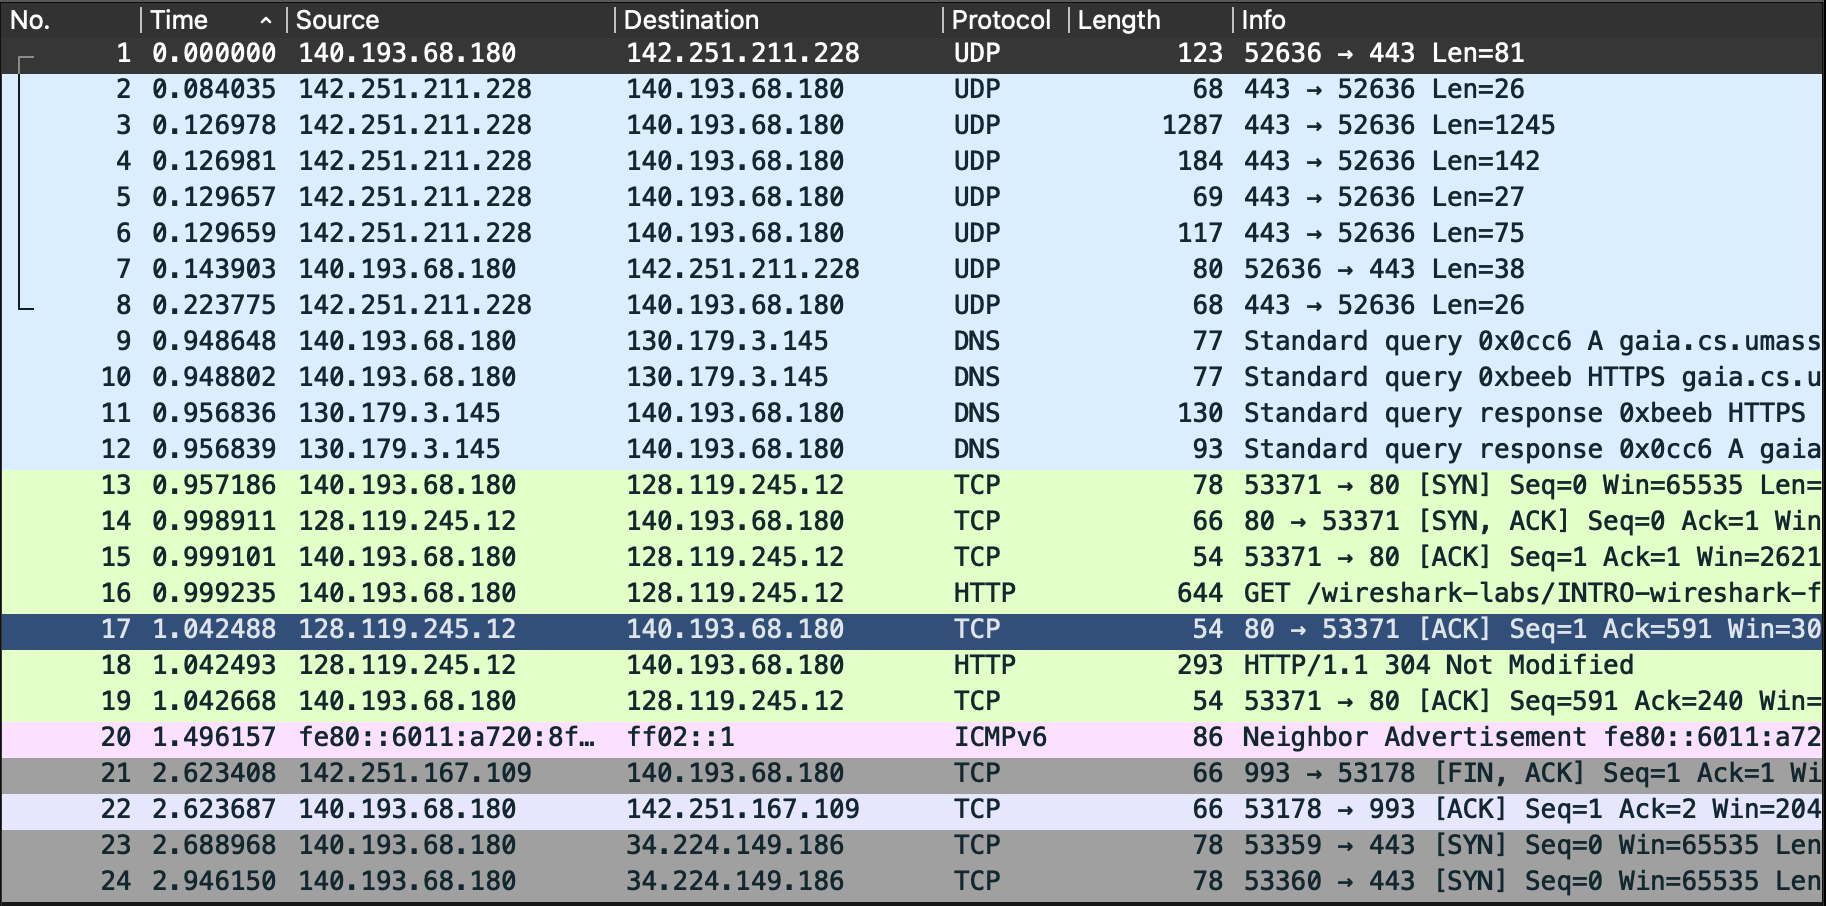
\includegraphics[width=0.8\textwidth]{p1_1}
        \caption{Packet-listing window}
        \label{fig:p1_1}
    \end{figure}


    \item The time taken for when the HTTP GET message was sent to when the HTTP OK reply was recieved was 0.04264 seconds. This was calculated by subtracting the time the HTTP GET message was sent from the time the HTTP OK reply was recieved. This can be seen in \autoref{fig:p1_2}.

    \begin{figure}[ht!]
        \centering
        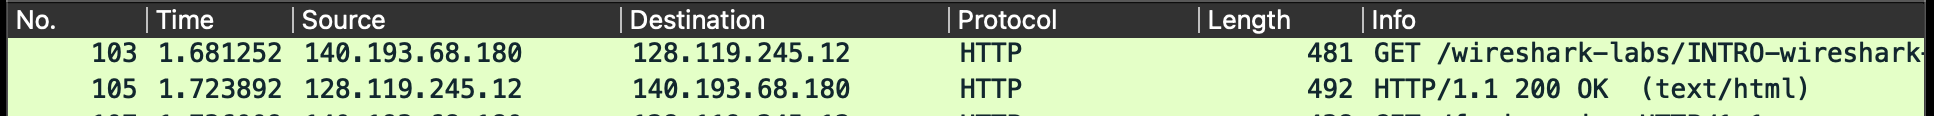
\includegraphics[width=0.8\textwidth]{p1_2}
        \caption{Time taken for HTTP GET message to HTTP OK reply}
        \label{fig:p1_2}
    \end{figure}

    \item The Internet address of the gaia.cs.umass.edu is 128.119.245.12 and the Internet address of my computer is 140.193.68.100. These addresses are sseen in \autoref{fig:p1_2}.
    
    \item Making 20 different requests and finding the delay between the HTTP GET message and the HTTP OK reply, the average delay was 0.08513 seconds. The plot of the 20 different requests can be seen in \autoref{fig:p1_3}.
    
    \begin{figure}[ht!]
        \centering
        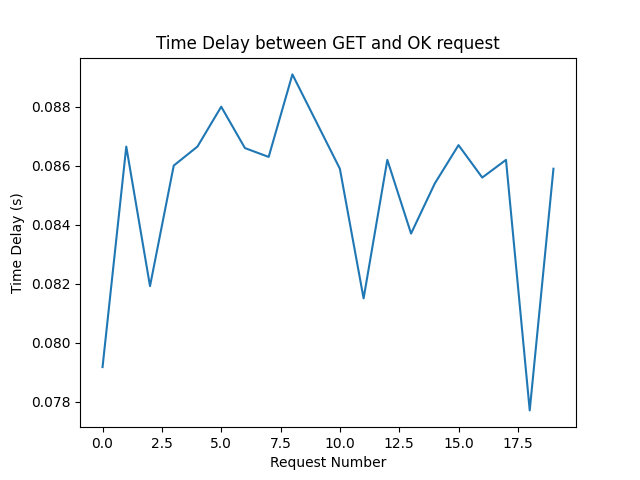
\includegraphics[width=0.8\textwidth]{p1_3}
        \caption{20 different requests}
        \label{fig:p1_3}
    \end{figure}
\end{enumerate}

\newpage
\section{Wireshark Lab: HTTP}

\begin{enumerate}
    \item The browser is running HTTP version 1.1 and so is the server. This can be deduced from the GET and OK requests both having HTTP/1.1 in the info column. As seen in \autoref{fig:p2_1}.
    \begin{figure}[ht!]
        \centering
        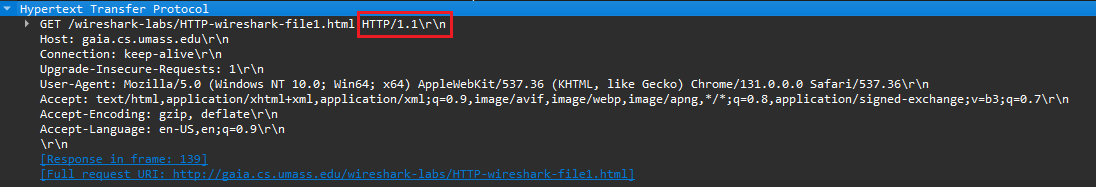
\includegraphics[width=0.8\textwidth]{p2_1}
        \caption{HTTP version}
        \label{fig:p2_1}
    \end{figure}
    \item The browser indicates it accepts en-US. As seen in \autoref{fig:p2_2}.
    \begin{figure}[ht!]
        \centering
        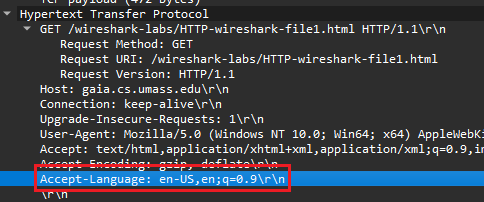
\includegraphics[width=0.35\textwidth]{p2_2}
        \caption{Accepted languages}
        \label{fig:p2_2}
    \end{figure}
    \newpage
    \item The IP address of my computer is 192.168.2.10 and the gaia.cs.umass.edu server is 128.119.245.12. This can be seen in the GET request and OK response. The source of the GET request is my computer and the destination is the server, vice-versa for the OK response. As seen in \autoref{fig:p2_3}.
    \begin{figure}[ht!]
        \centering
        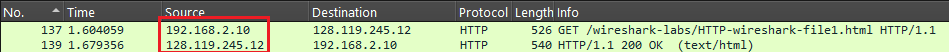
\includegraphics[width=0.6\textwidth]{p2_3}
        \caption{IP addresses}
        \label{fig:p2_3}
    \end{figure}
    \item The status code returned by the server is 200. This can be seen in the info column of the OK request, or the Hypertext Transfer Protocol section. As seen in \autoref{fig:p2_4}.
    \begin{figure}[ht!]
        \centering
        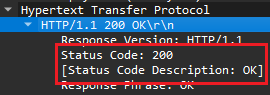
\includegraphics[width=0.6\textwidth]{p2_4}
        \caption{Status code}
        \label{fig:p2_4}
    \end{figure}
    \item The file was last modified at: January 24, 2025 at 6:59:01 GMT. This can be seen in OK response from the server in the Hypertext Transfer Protocol section. As seen in \autoref{fig:p2_5}.
    \begin{figure}[ht!]
        \centering
        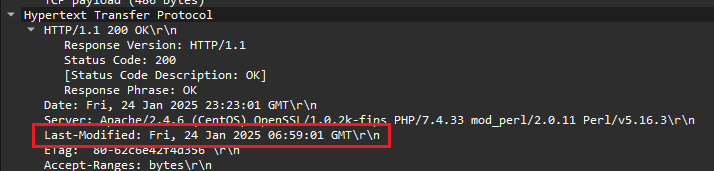
\includegraphics[width=0.6\textwidth]{p2_5}
        \caption{Last modified date}
        \label{fig:p2_5}
    \end{figure}
    \item 128 bytes of content was returned to the browser, and can be seen in the Content-Length field in the OK response. As seen in \autoref{fig:p2_6}.
    \begin{figure}[ht!]
        \centering
        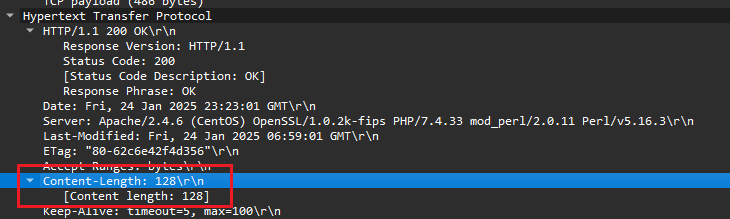
\includegraphics[width=0.4\textwidth]{p2_6}
        \caption{Content length}
        \label{fig:p2_6}
    \end{figure}

    \item The headings in the two windows are the same.
\end{enumerate}

\section{The HTTP CONDITIONAL GET/response interaction}
\begin{enumerate}
    \setcounter{enumi}{7}
    \item The first HTTP GET request does not have an If-Modified-Since header. 
    \item The server does explicitly return the contents of the file as we can see the text in the response to the first GET. It is 371 bytes and can be seen in the Hypertext Transfer Protocol section of the response.
    \begin{figure}[ht!]
        \centering
        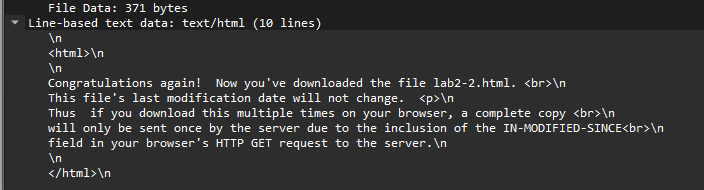
\includegraphics[width=0.6\textwidth]{p3_1}
        \caption{First HTTP GET request}
        \label{fig:p3_1}
    \end{figure}
    \item Inspecting the second HTTP GET request, we do see an If-Modified-Since header. The info followed by the header is ``If-Modified-Since: Tue, 23 Sep 2003 05:35:00 GMT$\backslash$r$\backslash$n''. This can be seen in the Hypertext Transfer Protocol section of the GET request.
    \begin{figure}[ht!]
        \centering
        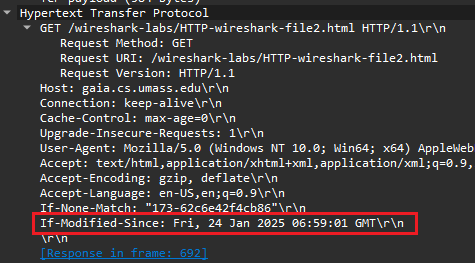
\includegraphics[width=0.6\textwidth]{p3_2}
        \caption{Second HTTP GET request}
        \label{fig:p3_2}
    \end{figure}
    \item The HTTP status code of is 304 with a response phrase of Not Modified. The server did not explicitly return the contents of the file as the browser already had the file cached. There is also no content length in the response 
    \begin{figure}[ht!]
        \centering
        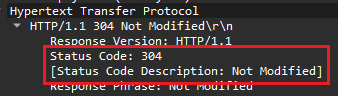
\includegraphics[width=0.6\textwidth]{p3_3}
        \caption{HTTP response}
        \label{fig:p3_3}
    \end{figure}
\end{enumerate}

\section{Retrieving Long Documents}
\begin{enumerate}
    \setcounter{enumi}{11}
    \item One HTTP GET request was sent by the browser. 
    \begin{figure}[ht!]
        \centering
        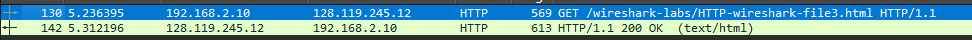
\includegraphics[width=0.6\textwidth]{p4_4}
        \caption{HTTP GET request}
        \label{fig:p4_0}
    \end{figure}
    \item Four TCP segments were needed to carry the single HTTP response message. In the response from the server, there is an entry stating 4 reassembled TCP segments.
    \begin{figure}[ht!]
        \centering
        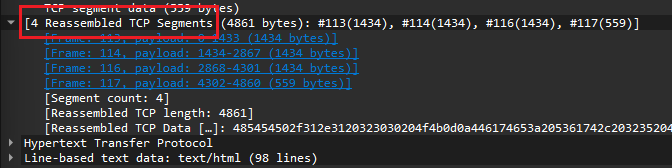
\includegraphics[width=0.6\textwidth]{p4_1}
        \caption{Reassembled TCP segments}
        \label{fig:p4_1}
    \end{figure}
    \item The status code and phrase associated with the response to the HTTP GET request is 200 OK.
    \begin{figure}[ht!]
        \centering
        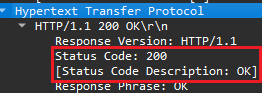
\includegraphics[width=0.6\textwidth]{p4_2}
        \caption{Status code and phrase}
        \label{fig:p4_2}
    \end{figure}
    \item There are three packets with status lines stating a continuation.
    \begin{figure}[ht!]
        \centering
        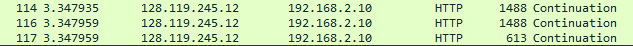
\includegraphics[width=0.6\textwidth]{p4_3}
        \caption{Continuation packets}
        \label{fig:p4_3}
    \end{figure}
\end{enumerate}

\section{HTML Documents with Embedded Objects}

\begin{enumerate}
    \setcounter{enumi}{15}
    \item 3 HTTP GET request messages were sent by the browser. One for the html and the other two for the image. The internet address of the first and second requests was: 128.119.245.12, and the third request was: 178.79.137.164.
    \begin{figure}[ht!]
        \centering
        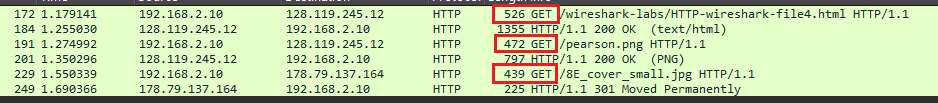
\includegraphics[width=0.6\textwidth]{p5_1}
        \caption{HTTP GET requests}
        \label{fig:p5_1}
    \end{figure}
    \item The requests for images are done in parallel. However in the packet capture the requests are done sequentially. The first request is for the html file, then we get an OK response. Then the browser sends a request for the first image, then we get an OK response. Then the browser sends a request for the second image, then we get an OK response. This can be seen in \autoref{fig:p5_1}. This could be due to the second image being larger than the first image, we are also getting a 301 response for the second image which could be causing the delay. In this case it seems the requests are done sequentially, but in a real world scenario the requests would be done in parallel.
\end{enumerate}

\section{HTTP Authentication}

\begin{enumerate}
    \setcounter{enumi}{17}
    \item In the initial HTTP GET request, the server responds with a 401 code and a message of Unauthorized. 
    \begin{figure}[ht!]
        \centering
        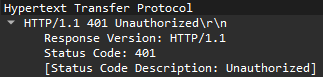
\includegraphics[width=0.6\textwidth]{p6_1}
        \caption{Initial HTTP GET request}
        \label{fig:p6_1}
    \end{figure}
    \item The new field in the second HTTP GET request is the Authorization field. It is a basic authentication field with the value encoded in base64.
    \begin{figure}[ht!]
        \centering
        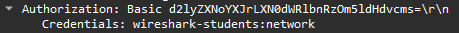
\includegraphics[width=0.6\textwidth]{p6_2}
        \caption{Second HTTP GET request}
        \label{fig:p6_2}
    \end{figure}
\end{enumerate}

\section{Additional Questions}
\begin{enumerate}
    \item In the TCP/IP stack, HTTP belongs in the application layer.
    \item The underlying transport layer protocol used by TCP is IP.
    \item The HTTP response for a successful request is 200 OK.
    \item When a file exceeds the payload size of a single packet, the file is split into multiple TCP segments and are sent individually. The segments are then reassembled at the destination.
    \item The components of the HTTP status line are the status code and the status phrase.
    \item The encoding method used in HTTP authentication is base64.
    \item Basic authentication is not secure as base64 can be easily decoded, allowing the information in the header to be read. If it contains sensitive information, it can be easily stolen. As well as, base64 is not an encryption method, it is an encoding method.
\end{enumerate}

% --------------------------------------------------------------------------------
% END BODY
% --------------------------------------------------------------------------------

\end{document}
